\section{Process model, multiplicity and the thermodynamic limit}
\label{sec:model}

\subsection{Reactor--jacket model and actuator}
The reactor hosts the irreversible first-order reaction $A\rightarrow B$ with rate $r_A=k_0\,e^{-E/(RT)}C_A$. With constant volumes and physical properties, the mass balance of $A$ and the energy balances of the reactor and of the jacket are
\begin{align}
\frac{dC_A}{dt} &= \frac{q}{V}\left(C_{Af}-C_A\right) - r_A, \label{eq:mass}\\
\frac{dT}{dt} &= \frac{q}{V}\left(T_f-T\right) + \frac{-\Delta H}{\rho c_p}\,r_A - \frac{UA}{V\rho c_p}\left(T-T_j\right), \label{eq:energy}\\
\frac{dT_j}{dt} &= \frac{q_j}{V_j}\left(T_{jf}-T_j\right) + \frac{UA}{V_j\rho_j c_{pj}}\left(T-T_j\right). \label{eq:jacket}
\end{align}
The manipulated variable is the coolant flow $q_j$; the measured outputs are $T$ and $T_j$. The valve is limited to $q_j\in[0,\umax]$~L/min and to a slew rate of $\slew$~L/min$^2$, and the controllers run with a zero-order hold at $\Delta t=\dtCtrl$~min \cite{hippe2006windup,tarbouriech2009antiwindup,choudhury2005modelling}. Table~\ref{tab:parameters} lists the parameters. The heat-transfer capacity $UA$ enters Eqs.~\eqref{eq:energy}--\eqref{eq:jacket} as a time-varying input, which is how fouling is introduced in Section~\ref{sec:fouling}; all other parameters are constant except where a disturbance is stated.

\begin{table*}[t]
\centering
\footnotesize
\caption{Model, actuator and sampling parameters.}
\label{tab:parameters}
\resizebox{\ifdim\width>\textwidth\textwidth\else\width\fi}{!}{%
\begin{tabular}{lc}
\toprule
Symbol & Value \\
\midrule
$q$, $V$, $V_j$ & 100 L/min, 100 L, 20 L \\
$k_0$, $E/R$ & 7.2e+10 min$^{-1}$, 8750 K \\
$-\Delta H$ & 5.0e+04 cal/mol \\
$\rho c_p$, $\rho_j c_{pj}$ & 500, 500 cal/(L K) \\
$UA_0$ & 5.0e+04 cal/(min K) \\
$C_{Af}$, $T_{jf}$ & 1.0 mol/L, 300 K \\
$T_f$ (nominal / cooled) & 350 / 320 K \\
$[u_{\min}, u_{\max}]$, slew & [0, 300] L/min, 80 L/min$^2$ \\
$\Delta t$ & 0.02 min \\
\bottomrule
\end{tabular}%
}
\end{table*}


Linearizing Eqs.~\eqref{eq:mass}--\eqref{eq:jacket} at an equilibrium $(\bar C_A,\bar T,\bar T_j,\bar q_j)$ gives $\dot{\mathbf{x}}=\mathbf{A}\mathbf{x}+\mathbf{b}\,q_j$ with
\begin{equation}
\mathbf{A}=\begin{bmatrix} a_{11} & a_{12} & 0\\ a_{21} & a_{22} & a_{23}\\ 0 & a_{32} & a_{33}\end{bmatrix},\qquad
\mathbf{b}=\begin{bmatrix}0\\0\\ b_3\end{bmatrix},\qquad b_3=\frac{T_{jf}-\bar T_j}{V_j}.
\label{eq:jacobian}
\end{equation}
The input enters only through the jacket, and its gain $b_3$ is proportional to the temperature difference between the coolant supply and the jacket. This structural fact will matter twice: for the cascade, whose slave loop acts on exactly this channel, and for fouling, which drives $\bar T_j$ towards $T_{jf}$ and therefore $b_3$ towards zero. The transfer function from $q_j$ to $T$ follows from Eq.~\eqref{eq:jacobian} as
\begin{equation}
G(s)=\frac{b_3\,a_{23}\,(s-a_{11})}{\det(s\mathbf{I}-\mathbf{A})},
\label{eq:gs}
\end{equation}
with a single zero at $s=a_{11}<0$.

\subsection{Van Heerden analysis and steady-state branches}
At steady state, the mass and jacket balances give
\begin{gather}
C_A(T)=\frac{qC_{Af}}{q+Vk(T)},\\
T_j(T,q_j)=\frac{q_jT_{jf}+(UA/\rho_jc_{pj})\,T}{q_j+UA/\rho_jc_{pj}}.
\end{gather}
Equilibria are the intersections of the heat generation and removal curves \cite{aris1958analysis,uppal1974dynamic,alvarez1995robust}
\begin{align}
Q_g(T) &= (-\Delta H)\,V\,k(T)\,C_A(T), \label{eq:qg}\\
Q_r(T,q_j) &= q\rho c_p\,(T-T_f) + UA\,\bigl(T-T_j(T,q_j)\bigr). \label{eq:qr}
\end{align}
An intersection at which $\partial Q_g/\partial T>\partial Q_r/\partial T$ violates the Van Heerden slope condition and is open-loop unstable \cite{seborg2010process,bequette2003process,luyben2007chemical}; the converse is necessary but not sufficient, so stability is always checked here on the spectrum of $\mathbf{A}$.

Figure~\ref{fig:van_heerden}(b) shows the equilibrium temperature versus coolant flow, computed by bracketing every sign change of $Q_g-Q_r$ on a fine temperature grid and refining it with Brent's method. With the nominal feed temperature, $T_f=\TfNom$~K, the curve is single-valued: over the whole valve range there is one equilibrium, and none of the sampled equilibria has an eigenvalue with positive real part (count of unstable points: $\nNomUnstable$). At the nominal flow of $\qjNom$~L/min the reactor sits at $\TNom$~K with $\convNom\%$ conversion and eigenvalues $\lamANom$, $\lamBNom$ and $\lamCNom$~min$^{-1}$.

Cooling the feed moves the generation curve with respect to the removal line. At $T_f=\TfSad$~K three equilibria coexist on the sampled grid for $q_j$ between $\qMultiLo$ and $\qMultiHi$~L/min. Placing the middle branch at $\bar T=\TSad$~K fixes $\bar C_A$ from the mass balance, $\bar T_j$ from Eq.~\eqref{eq:energy} and then $\bar q_j=\qjSad$~L/min from Eq.~\eqref{eq:jacket}; Powell's hybrid root finder started from this point returns it to machine precision. The three equilibria at this flow are listed in Table~\ref{tab:operating_points}: an extinguished state at $\TlowSad$~K (largest eigenvalue real part $\lamLow$~min$^{-1}$), the middle state at $\TSad$~K, and an ignited state at $\ThighSad$~K ($\lamHigh$~min$^{-1}$). The middle state has eigenvalues $+\lamASad$, $\lamBSad$ and $\lamCSad$~min$^{-1}$: one unstable direction, i.e.\ a saddle, with an unstable time constant $\tau_u=1/\lambda_1=\tauU$~min. Its conversion is $\convSad\%$, against $\convNom\%$ at the nominal point.

\begin{figure*}[t]
\centering
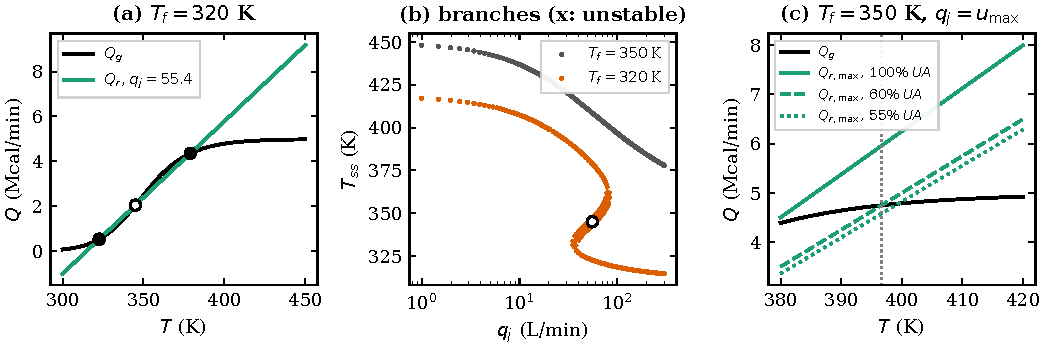
\includegraphics[width=\textwidth]{figures/fig1_van_heerden.pdf}
\caption{(a) Heat generation and removal at the saddle flow $q_j=\qjSad$~L/min and $T_f=\TfSad$~K; open marker: unstable equilibrium. (b) Equilibrium temperature versus coolant flow for the nominal and the cooled feed; crosses: open-loop unstable equilibria. (c) Heat generation and maximum heat removal ($q_j=u_{\max}$) at the nominal feed for three levels of $UA$; dotted line: nominal setpoint.}
\label{fig:van_heerden}
\end{figure*}

\begin{table*}[t]
\centering
\footnotesize
\caption{Operating points. Equilibria: number of steady states at the same $q_j$; $UA_{\mathrm{crit}}$: heat-transfer capacity below which holding $T$ needs $q_j > u_{\max}$ (Eq.~\eqref{eq:ua_crit}).}
\label{tab:operating_points}
\resizebox{\ifdim\width>\textwidth\textwidth\else\width\fi}{!}{%
\begin{tabular}{lcccccccc}
\toprule
Point & $T_f$ (K) & $q_j$ (L/min) & $T$ (K) & $C_A$ (mol/L) & $T_j$ (K) & $\lambda_{1,2,3}$ (min$^{-1}$) & Equilibria & $UA_{\mathrm{crit}}/UA_0$ (\%) \\
\midrule
Nominal & 350 & 100.00 & 396.65 & 0.0502 & 348.33 & -1.571, -11.801, -13.269 & 1 & 60.0 \\
Saddle & 320 & 55.38 & 345.00 & 0.5896 & 328.96 & 0.744, -0.903, -8.288 & 3 & 40.4 \\
\bottomrule
\end{tabular}%
}
\end{table*}


The open-loop phase portrait at the saddle flow, Fig.~\ref{fig:phase_portrait}, shows the separatrix behaviour reported by Uppal, Ray and Poore \cite{uppal1974dynamic}: of $\nPortrait$ initial conditions on a grid in the $(C_A,T)$ plane, $\nIgnite$ end on the ignited branch and the rest on the extinguished branch. A reactor operated at $\TSad$~K without feedback leaves the setpoint in either direction depending on the sign of the first perturbation, so any loss of feedback authority produces either ignition or extinction.

\begin{figure}[t]
\centering
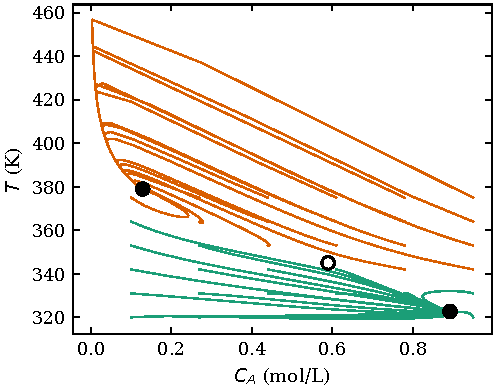
\includegraphics[width=\columnwidth]{figures/fig2_phase_portrait.pdf}
\caption{Open-loop trajectories at $q_j=\qjSad$~L/min, $T_f=\TfSad$~K, projected on the $(C_A,T)$ plane over 20~min. Orange: trajectories ending on the ignited branch; green: on the extinguished branch. Open marker: saddle at $\TSad$~K.}
\label{fig:phase_portrait}
\end{figure}

\subsection{Thermodynamic controllability limit}
Feedback can move an equilibrium but cannot create cooling capacity. If the temperature and the concentration are held at their setpoint values, the heat that must leave through the wall,
\begin{equation}
Q_{\mathrm{load}} = V\rho c_p\left[\frac{q}{V}\left(T_f-\bar T\right)+\frac{-\Delta H}{\rho c_p}\,r_A(\bar C_A,\bar T)\right],
\end{equation}
does not depend on $UA$. The jacket temperature that removes it is $\bar T_j=\bar T-Q_{\mathrm{load}}/UA$, and the jacket balance then gives the required flow $q_j=Q_{\mathrm{load}}/\left[\rho_jc_{pj}(\bar T_j-T_{jf})\right]$. Setting $q_j=u_{\max}$ yields the critical heat-transfer capacity
\begin{equation}
UA_{\mathrm{crit}} = \frac{Q_{\mathrm{load}}}{\bar T - T_{jf} - Q_{\mathrm{load}}/(\rho_jc_{pj}\,u_{\max})},
\label{eq:ua_crit}
\end{equation}
below which no controller acting on this valve can hold the setpoint. Equivalently, $UA<UA_{\mathrm{crit}}$ is the condition $Q_g(\bar T)>Q_{r,\max}(\bar T)$, with $Q_{r,\max}(T)=Q_r(T,u_{\max})$.

At the nominal point Eq.~\eqref{eq:ua_crit} gives $UA_{\mathrm{crit}}=\fcritNom\%$ of the clean value. The heat generated at the setpoint is $Q_g=\QgNom$~Mcal/min. With a clean jacket and the valve fully open the reactor could remove $Q_{r,\max}=\QrMaxFull$~Mcal/min; at $60\%\,UA$ the maximum removal is $\QrMaxSixty$~Mcal/min, equal to the generation within the printed precision, so $60\%$ is the boundary itself; at $55\%\,UA$ it drops to $\QrMaxFiftyFive$~Mcal/min, below $Q_g$. Figure~\ref{fig:van_heerden}(c) shows the corresponding curves: at $55\%\,UA$ the maximum-removal curve crosses the generation curve above the setpoint, so the hottest equilibrium the valve can hold is above $\TNom$~K. This is a property of the plant and the valve and holds for every control law. At the saddle the same formula gives $UA_{\mathrm{crit}}=\fcritSad\%$ (Table~\ref{tab:operating_points}): the cooled-feed point needs less heat removal and has more margin against fouling, a margin that will turn out to be unusable with fixed gains (Section~\ref{subsec:res_fouling}).
